\section{Vision}

The vision system is aimed to be a simple and robust platform, providing the latest world description. A requirement for the vision system was to avoid increasing the delay caused by the video feed. The initial world model will be passed to the predictor, which will smooth out the vision output and buffer object positions. This keeps record of object locations, should it be impossible to detect it in a few following frames, and also avoids confusing the planner with erratic object movement from false detections. The resulting world model is then transmitted to the planner in control of the robots. The vision system includes several calibration routines, and saves configurations per pitch room and computer used for accessing the vision feed.

\subsection{Approach}

The vision system is common for both groups in the team. It was developed by Group 12 and augmented with ideas from Group 11's initial vision platform. 

The vision uses a HSV (hue, saturation, value) coded frame rather than the default BGR (blue, green, red). This separates the kind of colour from its intensity and brightness. When a frame is captured, first the radial distortion is removed, allowing object positions to be directly mapped for the planner. Then, blur is applied to the image, simplifying colour clusters, causing objects to become more "connected" and thus easier to identify. The frame is then converted to HSV and all future processing will take place over the HSV frame.

The main approach of the vision system is to detect clusters of colour. Examples of this include yellow and blue clusters signifying the centres of robots and a suitably sized red cluster being the ball. For each colour, clusters are detected by creating a mask based on configured thresholds, and finding contours within that mask. In case more than two objects of the same type are detected, only the best match is taken. Potential robots are identified by a yellow or a blue cluster being the centre dot of a robot. After a potential robot centre is identified, green and pink colour clusters are detected in a 40x40 pixel area around the centre. The existence of the pink and green clusters confirm the detected centre indeed being a robot. If none are found, then this robot centre is deemed a false positive and skipped, detection continues with the next best central cluster.  Following verification, the robot is identified within the yellow/blue team by the count of the aforementioned pink dots: If we find three pink clusters, then the robots is the pink team member, otherwise it is the green team member. The pink dots on a green top plate were significantly easier to detect than the green dots, and thus chosen for identification.

Once the robot is identified as the pink/green member of the yellow/blue team, the system determines the orientation of the robot. This is done by constructing a vector from the back left dot (pink circle for green robot; green circle for pink robot) to the robot centre, and corrected by around 45 degrees counter-clockwise. The correction amount is dynamically configurable to allow for differences in dot positions on the top plates.

For the ball positioning, the largest red cluster is taken. Ball movement is determined by the time difference between the frames and the last known ball position: a vector is constructed from the previous position to the current position. Velocities of all objects are calculated relative to the movement from the previous frame. 

Colour thresholding can become unreliable if the thresholds are not perfectly adjusted, or the environment (e.g. lighting conditions) changes. If the vision system behaves in an unexpected manner, it needs to be recalibrated.


\subsection{Semi-Automatic Calibration}

The vision system has several calibration routines, most importantly a colour calibrator. 

The colour calibration routine is, by default, run every time the vision system is started, but can be skipped, defaulting to the last saved configuration. 
The vision platform will prompt the user to click on objects of each of the relevant colours in sequence. Predefined hue ranges for the colours distinguished are shown in \autoref{fig:hues}. On every click, a 3x3 square of pixels around the click is extracted, and the pixels within a predefined hue range (hard coded for each colour) are recorded.
The thresholds for saturation and value are formed using the according minimum values of relevant recorded pixels as the lower bound, and the maximum absolute value (255) as the upper bound.
This worked more reliably than extracting the maximum from the clicked areas as well.

This makes it easy to recalibrate the whole vision system on each launch to adapt to environment changes.

\begin{figure}[H]
\centering
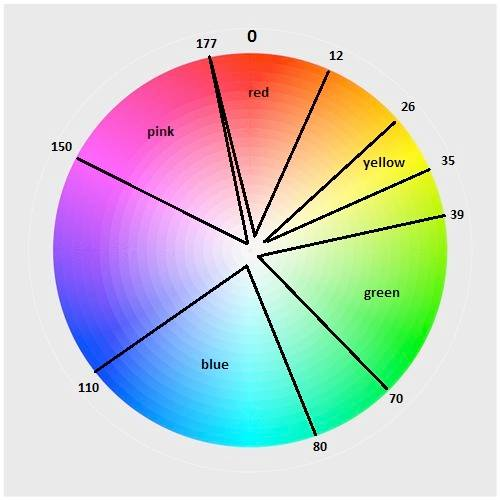
\includegraphics[scale=0.5]{vision_hue}
\caption{Predefined Hue Ranges}
\label{fig:hues}
\end{figure}

\subsection{Manual Calibration}
The platform implements a manual way of determining threshold values for colour filters, as well as a pitch cropping specification routine.

The vision system GUI offers sliders to manually determine the threshold values for the colour masks. This is useful for debugging and initial calibration of the colours.

The cropping calibration, which is by default disabled (trigger in the vision code is commented out) determines which parts of the vision feed to use. This has to be run very rarely - once for each camera after every change in the camera angle or position. This provides a quick and efficient way of correcting the pitch area and ignoring any outlying distractions.
